%************************************************
\chapter{An evolutionary algorithm for inverse folding inspired by Lévy flights.}\label{ch:arnaque}

In the previous chapter of our work, we prevented the RNA design as an optimization problem and provided a significant literature review on the existing tools addressing that problem. We highlighted some limitations of the existing tools, particularly the ones implementing evolutionary algorithms. One of the evolutionary algorithms' main challenges is to avoid deception, which is the fast convergence to a local optimum. Most evolutionary algorithms' early convergence to a local optimum is due to the local search implementation, which is the consequence of the local mutation scheme. 

An alternative mutation scheme to the classical local search is the Lévy mutation to avoid this pitfall. We propose an evolutionary algorithm implementing a similar Lévy mutation in this chapter but adjusted to the RNA design problem. Our implementation, called \texttt{aRNAque} is available on GitHub as a python script. Compared to existing inverse folding tools, the benchmark results show improved performance on both pseudoknot-free and pseudoknotted datasets.
	
\section{Material and methods}

This section provides a detailed description of \texttt{aRNAque} algorithm in general and in particular the Lévy mutation scheme implemented. 

\subsection{\texttt{aRNAque}'s mutation operator}

For a given target RNA secondary structure in its string representation $\sigma^*$ of length $L$, the space of potential solutions to the inverse folding problem is $\{\text{A},\text{C},\text{ G}, \text{U}\}^L$.
An evolutionary algorithm explores the space of solutions through its move (or mutation) operator. To explore the search space of compatible sequences (sequences with canonical base pairs at the corresponding open and closed bracket positions) with $\sigma^*$ exclusively, we propose a mutation step that depends on the nucleotide canonical base pair probability distribution.

Let~\(\mathcal{N}= \big \{ \text{A},\text{C},\text{ G}, \text{U} \big \}\) be the set of nucleotides weighted respectively by the probabilities:
\begin{equation*}
P_{\mathcal{N}} = \big \{ w_{\text{A}}, w_{\text{C}}, w_{\text{U}}, w_{\text{G}} \big\}
\end{equation*}
and~\(\mathcal{C} = \big \{ \text{AU}, \text{UA}, \text{ CG}, \text{GC}, \text{UG}, \text{GU}\big \}\)~be the set of canonical base pairs weighted respectively by the probabilities:
\begin{equation*}
P_{\mathcal{C}} = \big \{w_\text{AU}, w_\text{UA}, w_\text{ CG}, w_\text{GC}, w_\text{UG}, w_\text{GU} \big \} 
\end{equation*}
where
\begin{equation*}
\sum P_{\mathcal{N}} = 1, \sum P_{\mathcal{C}}  = 1 
\end{equation*}
%and
%\begin{equation*}
%P_{AU} = P_{UA}, P_{UG} =P_{GU}, P_{CG} = P_{GC}
%\end{equation*}
Our evolutionary algorithm relies on the flexibility of the mutation parameters $P_{\mathcal{N}}, P_{\mathcal{C}}$. These parameters allow explicit control of the GC-content of the RNA sequences during the designing procedure.

 We examined the binomial and Zipf distributions:

\begin{itemize}
	\item Binomial mutation: here $U$ has a binomial distribution: 
	$$
	P(U=n)= \binom{L}{n} \mu^n (1-\mu)^{L-n}
	$$
	for some $0 \leq \mu \leq 1$, such that $u=\mu \cdot L$. We can think of this mutation mode arising from each nucleotide of an RNA sequence independently undergoing a point mutation with probability $\mu$, i.e. $\mu$ is the per-nucleotide or point mutation rate. 
	
	\item Lévy mutation: $U$ has a Zipf distribution given by: 
	$$
	P(U=n)= \frac{1/n^c}{ \sum_{k=1}^{L}{1/k^c}}
	$$
	where $c>0$ is the value of the exponent characterizing the distribution.
\end{itemize}

Figure \ref{Fig:histomut} shows the distribution of the number of point mutations on a sequence of length $88$ nucleotides for both mutation schemes. Both distributions have the same mean, and the difference between the two distributions is more perceptible on their tails. 

In the rest of this work, a local mutation will refer to a binomial mutation with parameter $\mu \approx 1/L$.

\begin{figure*}[ht]
	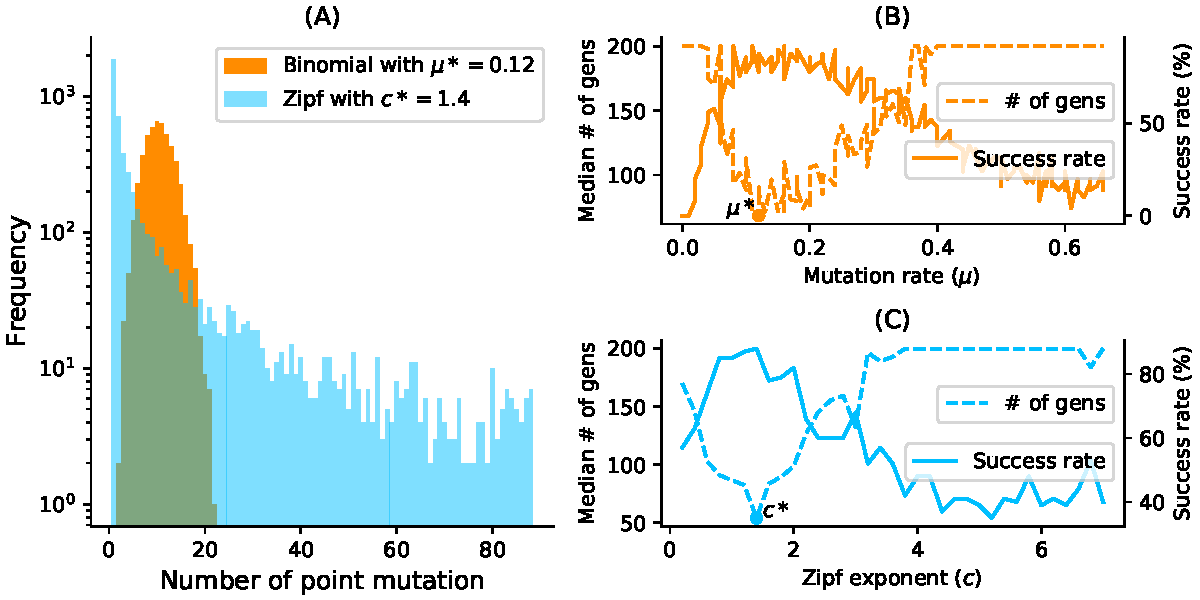
\includegraphics[width=1.0 \linewidth]{../res/images/arnaque/fig1.pdf}
	\caption{ \textbf{Binomial \emph{vs.} Zipf distributions.} (A) Samplings Binomial and Zipf distributions for the best binomial mutation rate $\mu^*$ (respectively $c^*$ for the best Zipf exponent parameter). Both distributions have a mean of $8.7$ point mutations for a sequence of length $88$ nucleotides. (B) Tuning of binomial mutation rate parameter. For each $\mu \in [0,1]$ with a step size of $0.005$ and the pseudoknotted target \texttt{PKB00342} of length $88$, $50$ sequences were designed using \texttt{aRNAque}. (B) shows the median generations and the success percentage \emph{vs.} the mutation rate ($\mu$). The best mutation rate is $\mu^*=0.085$ (with a median number of generation $93.5$ and a success rate of $92\%$). (C) Tuning of Levy exponent. Similar to (B), for each $c \in [0,7]$ with a step size of $0.1$ and for the same pseudoknotted target structure, $100$ sequences were designed using \texttt{aRNAque}. It shows the median generations and the percentage of success \emph{vs.} the exponent parameter ($c$). The Zipf exponent distribution that produced the highest success rate and the minimum number of generations is $c^*=1.4$.}\label{Fig:histomut}. 
\end{figure*}
We present the mutation algorithm in Algorithm \ref{Algo:Lévy}.

\begin{algorithm}
	\tcc{$P'=\{\phi'_1\dots \phi'_n\}$: the mutated population\; 
	$P= \{\phi_1\dots \phi_n\}$: a list of $n$ RNA sequences to mutate\;
	$P_{\mathcal{C}}=\{w_\text{AU}, w_\text{UA}, w_\text{ CG}, w_\text{GC}, w_\text{UG}, w_\text{GU}\}$: a vector containing the weights associated with each canonical base pairs\;
	$P_{\mathcal{N}}=\{w_\text{A}, w_\text{U}, w_\text{C}, w_\text{G} \}$: a vector containing the weights associated with each nucleotide\;
	$\mathcal{D}$: a given probability distribution (Lévy or Binomial) with parameter $p$ and $L$. Where $L$ is the length of the target RNA structure}
\KwInput{$P$, $\mathcal{D}(p, L)$, $P_{\mathcal{C}}$,  $P_{\mathcal{N}}$}
\KwOutput{$P'$} 
$ \{B_i\} \sim \mathcal{D}(p,L)$, where $i\in \{1,2,\dots,n\}$ \tcp*{Draw $n$ random numbers that follows a given distribution $\mathcal{D} (p,L)$ (Lévy or Binomial). $B_i$ is the number base pairs to mutate}
$\{U_i\} \sim \mathcal{D}(p,L)$, where $i\in \{1,2,\dots,n\}$ \tcp*{Draw $n$ random numbers that follows the same distribution as $B_i$ (Lévy or Binomial). $U_i$ is the number non base pair positions to mutate}

\For{ $i \in \{1, 2, \dots, n\}$ }{
	$\phi'\leftarrow P_i$ \tcp*{Assign the sequence $\phi_i \in P$ to $\phi'$ }
	\For{ $j \in \{1,2,...U_i\}$}{
		$r \in \{1,2,\dots, L\} \sim \mathcal{U}$ \tcp*{select uniformly a random position in the RNA sequence $\phi'$}
		$n_j \in \{\text{A}, \text{U}, \text{C}, \text{G}\} \sim P_{\mathcal{N}}$ \tcp*{select a random nucleotide $n_j$ with respect to $P_{\mathcal{N}}$} 
		$\phi'_r \leftarrow n_{j}$ \tcp*{replace the nucleotide at position $j$ in the RNA sequence $\phi'$ with $n_j$}
	}
	\For{ $j \in \{1,2,...B_i\}$}{
		$k_j \in \{\text{AU}, \text{UA}, \text{ CG}, \text{GC}, \text{UG}, \text{GU}\} \sim P_{\mathcal{C}}$ \tcp*{select a random base pair $k_{i}$ with respect to $P_{\mathcal{C}}$}
		$b \in \{(b_1,b_2)_i\} \sim \mathcal{U}$ \tcp*{select uniformly a random pair of base pair positions}
		$\phi'_b \leftarrow k_{j}$ \tcp*{replace respectively the nucleotides at the base pair position $b_i \in b$ by $k \in k_j$}
		
	}
	$P' \gets P'\cup \phi'$ \tcp*{Add $\phi'$ to the list $P'$}
}
	\caption{\texttt{aRNAque}'s mutation algorithm}\label{Algo:Lévy}
\end{algorithm}
%In addition to the two main features mentioned above, we also provide a web-server integrating an enriching interface to compare and analyse the designed sequences.

%%%%%%%%%%%%%%%%%%%%%%%%%%%%%%%%%%%%%%%%%%%%%%
%%                                          %%
%% Backmatter begins here                   %%
%%                                          %%
%%%%%%%%%%%%%%%%%%%%%%%%%%%%%%%%%%%%%%%%%%%%%%

\subsection{\texttt{aRNAque}'s objection functions}
\label{sec:objective_function}
Our EA reaches its performance through the minimization of three objective functions:

\begin{itemize}
	%\tightlist
	\item
	Hamming distance from the target structure: Since the main goal of the inverse folding problem is to find sequences that fold into a given target secondary structure~\(\sigma^*\), the simple fitness measurement~\(f\) of an RNA sequence~\(\phi\)~can be defined as follows:
\begin{equation}
\label{eq:fitness}
f(\phi, \sigma^*) = \frac{1}{1 + d_h(\sigma^{MFE}(\phi) , \sigma^*)}
\end{equation}

where~\(d_h(\cdot,\cdot)\)~is the hamming distance on the structure space (structures are in dot and bracket representation) defined in Equation \ref{eq:hamming}.

	%\tightlist
	\item
	Normalized Energy Distance (NED): It is used to minimize the free energy of the designed sequences. (See Equation \ref{ned} )

	\item
	Ensemble defect (ED) \cite{zadeh2011nucleic}: Here, we use the ED as a second objective function for refinement after having at least one sequence that folds into the target in the current population. It is defined in Equation \ref{ed}.
\end{itemize}
To minimize the NED and the hamming distance of a population of RNA sequences, instead of combining both measurements to form a multi-objective function, we use them separately at a different level of our EA. We use the NED as a selection weight for the sequences that will be mutated, and the hamming distance is used as a weight to elite ten best sequences that will always move to the next generation. Therefore the selection method we use is the \textit{fitness proportionate selection}, also known as roulette wheel selection \cite{lipowski2012roulette}. Once we have at least one sequence that folds into the given target in the current population (for the successful case), we start a random walk in its neutral network by minimizing the ensemble defect function (Eq. (\ref{ed})). The next section provides more detailed information about the core of our EA and the full pseudo-code. 

\subsection{\texttt{aRNAque}'s EA}

For a given population size $n$ and a target structure $\mathcal{S}^*$ of length $L$, an initial population $P$ is generated randomly as follows: 

\begin{enumerate}
	\item Select randomly $L$ nucleotides in $\mathcal{N}$
	
	\item Identify the base pair position $(i,j)$ in the random sequence, select randomly a base pair in the set of canonical base pairs $\mathcal{C}$ and fix the first nucleotide of the selected canonical base pair at the position $i$ and the second at position $j$.
	
	\item  Repeat 2. for all base pair positions in the target structure
	
	\item Repeat 1. 2. and 3. $n-$times.
\end{enumerate}
Let \(T\) be the maximum number of generations and \(F_t\) the set of all sequences found at a given time ~\(t\). After the initial population of RNA sequences is generated, our algorithm is described in Algorithm \ref{algo_desc}. The stopping criteria are two: 1) the number of generations ($t$) is equal to the max number of generations ($T$) or 2) the minimum hamming (or base pair) distance of the best RNA sequence solution to the target is $0$ (i.e the maximum fitness value is $1$ ).
\vspace{0.05cm}
\begin{algorithm}
	\tcc{$P'=\{\phi'_1\dots \phi'_n\}$: the best population\; 
		$P= \{\phi_1\dots \phi_n\}$: the initial population of $n$ RNA sequences\;
		$P_{\mathcal{C}}=\{w_{AU},w_{GU},w_{GC}\}$: a vector containing the weights associated with each base pair\;
		$P_{\mathcal{N}}=\{w_{A},w_{U},w_{C}, w_{G}\}$: a vector containing the weights associated with each nucleotide\;
		$\mathcal{D}$: a given probability distribution (L\'evy or Binomial) with parameter $p$ and $L$, where $L$ is the length of the target RNA structure\; 
		$T$: the maximum number of generations\; 
		$n$: the population size \; 
		$f(;)$: the fitness function used. It can be the hamming, base-pair or energy distance\;
		$\sigma^*$: the target structure in its string representation\; 
		$\mathcal{P}$: the energy parameters used for the folding}
	
	\KwInput{ $n$, $T$, $P_{\mathcal{N}}$,$P_{\mathcal{C}}$, $P$, $\mathcal{D}(p, L), f(;), \sigma^*, \mathcal{P}$}
	\KwOutput{Best population $P'$ }
	$P'\leftarrow P$ \tcp*{Assign the initial population to the best population }
	$t\leftarrow 0$ \tcp*{Initialize the number of generations to $0$ }
	
	\While{$t \leq T  \And f(\sigma^{MFE}(\phi_b), \sigma^*) \neq 1$ } {
		$\Sigma \gets \{\arg \min_{\sigma \in \Sigma} \Delta G(\phi_i, \sigma,\mathcal{P})\}$, \tcp*{Fold each sequence $\phi_i \in P'$ and store them in $\Sigma$.   Where $i\in \{1,2,\dots,n\}$, $\Gamma$ the structural ensemble and $\Delta G(\phi_i, \sigma)$ the free energy computed using the parameters $\mathcal{P}$}
		
		$\kappa = \lfloor (n\times0.1) \rfloor$ \tcp*{The number of RNA sequences to copy in the next generation without mutating them.}
		$F \leftarrow \{f(\sigma,\sigma^*) | \forall \sigma \in \Sigma\} $ \tcp*{Evaluate the fitnesses of the folded population to the target strucre $\sigma^*$ and store them in a list $F$}
		$E_{\kappa} \leftarrow \{\phi_1\dots \phi_{\kappa}\} \sim F$ \tcp*{copy of the $10\%$ best sequence based on their fitnesses $F$.} 
		
		$P_S \leftarrow \{\phi_i\} \sim F$, where $i\in \{1,2,\dots,n-\kappa\}$\ \tcp*{Randomly sample $(n-\kappa)$ RNA sequences from $P'$ with respect to their fitnesses $F$.}
		
		$M\leftarrow \texttt{mutate}(P_S, \mathcal{D}(p, L), P_{\mathcal{C}},  P_{\mathcal{N}})$ \tcp*{ Mutated the selected sequences using the mutation algorithm presented in the main text in out paper.}
		
		$P_b \gets M \cup E_{\kappa}$\tcp*{Combine the mutated population and the best solutions to form the new population that will be evolved in the next generation}
		$\phi_b \leftarrow \arg \max_{\mathcal{S} \in \Sigma} f(\sigma, \sigma^*)$\;
		$ t \gets t + 1$ \tcp*{Increment the time step (the number of generations)}
	}
	
	\caption{\texttt{aRNAque}}\label{main_EA}
\end{algorithm}

\subsection{Benchmark parameters and protocols}
For the benchmark results presented in this work, we use three datasets: the \texttt{Eterna100} dataset, \texttt{RFAM} dataset and \texttt{PseudoBase++} dataset. Depending on the datasets, a specific RNA folding tool is used. This section gives more details about \texttt{aRNAque}'s parameters, energy parameters and other tools parameters used for the benchmark results presented in this chapter. 
\subsubsection*{Folding tools}
Two tools for pseudoknotted RNA folding are considered in this work: \texttt{HotKnots} and \texttt{IPknot}. For pseudoknot-free RNA folding, we used \texttt{RNAfold}.
 For the mutation parameter and GC-content analysis presented in our work, we used \texttt{IPknot}, and both \texttt{HotKnots} and \texttt{IPknot} for \texttt{PseudobBse++} benchmarks. To be able to use \texttt{HotKnots} in \texttt{aRNAque} without copying \texttt{aRNAque} in the bin directory of \texttt{Hotknots}, we have performed some modifications on \texttt{Hotknots} source code. Details on the modifications are provided in the supplementary material SI 6. Furthermore, we considered \texttt{pkiss}, a well known tool for K-type pseudoknot prediction, but since the \texttt{PseudoBase++} dataset contains just $4$ K-type pseudoknotted structures and \texttt{pKiss} has higher time complexity ($O(n^6)$), we did not find it efficient for the benchmark we performed.
\subsubsection*{Mutation parameters tuning}
The main challenge for an evolutionary algorithm is to find optimum parameters such as mutation rate, population size and selection function.
We used $80$ pseudoknotted targets with lengths from $25$ to $181$ nucleotides for the mutation parameter analysis. We set the maximum number of generations $T$ to $200$ and the population size $n$ to $100$. The stopping criteria are two: 1) the number of generations ($t$) is equal to the max number of generations ($T$) or 2)the minimum hamming (or base pair) distance of the best RNA sequence solution to the target is $0$. The best mutation parameters ($c^*$ for Levy and $\mu^*$ for Binomial) are those that have the lowest median number of generations. The best mutation parameters obtained for both binomial and Lévy mutation modes are used to benchmark and compare the results on the entire datasets of RNA structures.
\subsubsection*{Benchmark on the \texttt{PseudoBase++} dataset}
Four benchmarks are performed on the pseudoknotted dataset: 1) mutation parameter analysis, 2) the GC-content and diversity analysis, 3) Local search versus Lévy search, 4) \texttt{aRNAque} (Lévy search) versus \texttt{antaRNA}. For the \texttt{aRNAque} (Binomial and Lévy) case, the four benchmarks share the same number maximum number of generations ($T=200$), population size ($n=100$), stopping criteria ($t=T$ or min fitness equals $0$).
For the \texttt{antaRNA} benchmark, the maximum number of iterations was set to $1200$, and a slight modification was made to allow the support of the folding tool $\texttt{HotKnots}$ (See Appendix 6).  
For booth tools and each benchmark,  $20$ runs were launched independently in parallel on a computer with the same resources, resulting in $20$ designed sequences per pseudoknotted target structure. To measure the performance of each tool, each designed sequence $s$ is folded into a secondary structure $\mathcal{S}$ and the similarities between $\mathcal{S}$ and $\mathcal{S}^*$ are computed using the base pair distance. 
For the GC-content benchmark, four GC-content values are considered, $\{0.25, 0.5, 0.75,1\}$ and the setting of each tool remains the same.
\subsubsection*{Benchmark on the \texttt{Eterna100} dataset}
We performed two benchmarks are one the \texttt{Eterna100} dataset: 1) a benchmark on the \texttt{Eterna100-V1} dataset using the \texttt{Turner1999} energy parameter and the both versions of \texttt{aRNAque} (one point and Lévy mutation), 2)a benchmark on the \texttt{Eterna100-V2} dataset using the \texttt{Turner2004} energy parameter and both versions of \texttt{aRNAque} (one point and Lévy mutation).
For each of the \texttt{Eterna100} benchmark we used the same evolutionary algorithm parameters; a maximum of $T=5000$ generations (i.e. a maximum of  $500,000$ evaluations), a population size of $n=100$ and the same stopping criteria (the number of generation $t=T$ or min fitness equals $0$). For both local and Lévy search, $5$ runs were launched independently, which results in $5$ designed sequences per target. We define success rate simply as the number of successfully designed targets. A target is considered successfully designed when at least one of the designed sequences folds into the target structure. 

For the benchmarks peformed on \texttt{ERD}, \texttt{NUPACK}, and \texttt{SentRNA} the default parameters were used. For \texttt{NEMO}, the number of iteration was set to $2500$ and for \texttt{RNAinverse} the objective function was set to be the partition function and the number of iteration at $1200$. 
\subsubsection*{Benchmark on the \texttt{non-Eterna100} dataset}
For the \texttt{non-EteRNA} dataset,  only the Turner2004 energy parameters were used. The maximum number of generations was set to be~\(5000\). The mutation parameters (~\(P_{\mathcal{C}}\)~and~\(P_{\mathcal{N}}\)) were chosen to be close to the nucleotide distribution of the RNA sequence in nature \cite{esmaili2015erd}.  

\begin{figure*}[t!]
	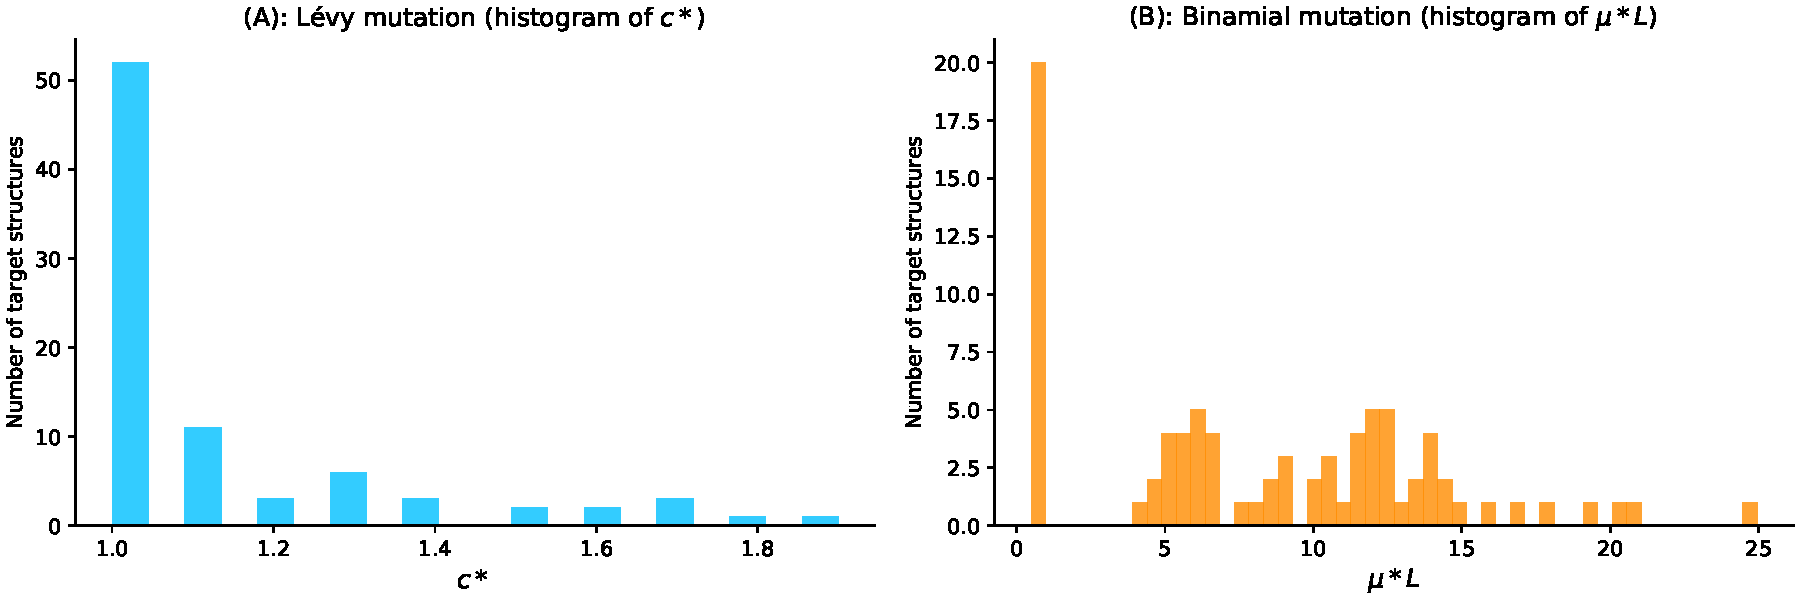
\includegraphics[width=1.0 \linewidth]{../res/images/arnaque/fig3.pdf}
	\caption{\textbf{Parameter tuning for both binomial and Lévy mutation schemes}. (A) Lévy mutation parameter tuning. Histogram of best exponent parameter ($c^*$) for a set of $81$ target structures with different pseudoknot patterns and various lengths. The most frequent best exponent value is $1$. (B) Binomial parameter tuning. Histogram of best mutation rate ($\mu^*$) for the same set of $81$ target structures with different pseudoknots and various lengths. The most frequent best parameter is the low mutation rate ($\approx 1/L$). For some structures, the best mutation rate is the high one for different lengths as well.} \label{Fig:tunning}
\end{figure*}
\section{Experimental results}


\subsection{\texttt{aRNAque}'s performance on pseudoknot-free target structures }
We compared the performance of \texttt{aRNAque} for pseudoknot-free target using the benchmark datasets: the non-\texttt{Eterna100} and the \texttt{Eterna100}. This subsection presents the statistical results obtained compared to benchmarked existing tools and the results found in the literature. In addition, we compared the performance of \texttt{aRNAque} (Lévy mutation) to the one of Ivry et al. \cite{ivry2009image} on a tripod pseudoknot-free RNA secondary structure.

\begin{figure*}[ht]
	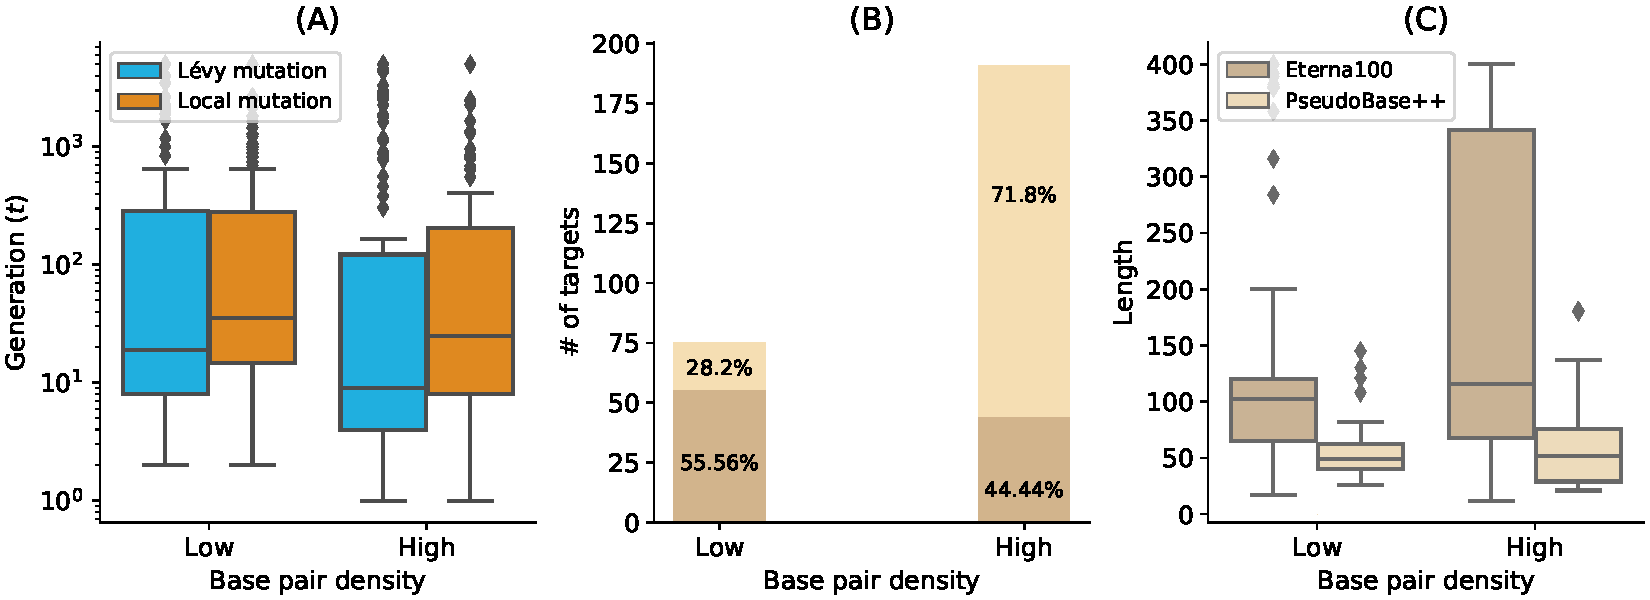
\includegraphics[width=1.\linewidth]{../res/images/arnaque/fig10.pdf}
	\caption{\textbf{Lévy mutation \emph{vs.} Local mutation: performance analysis with respect to the base-pair density}. The higher the base-pair density is, the more useful the Lévy mutation scheme to speed up the optimization EA. (A) Distributions of number of generations for the low and high base-pair density targets of the \texttt{Eterna100} dataset. (B) Percentages of targets with low and high base-pair density for the \texttt{Eterna100} and \texttt{PseudBase++}. (C) The length distributions of the low and high base-pair density pseudoknot-free and pseudoknotted targets.} \label{Fig:eterna_performance}
\end{figure*}  

\subsubsection{Performance on \texttt{Eterna100} dataset}

A first benchmark was performed on the \texttt{Eterna100} datasets. First, on the \texttt{Eterna100-V1} dataset, the Lévy flight version of \texttt{aRNAque} successfully designed $89\%$ of the targets and the one-point mutation (local mutation) version achieved $91\%$ of success, suggesting that for some target structures, local mutation can outperform the Lévy mutation scheme. Combining the two solutions, \texttt{aRNAque} solved in total $92\%$ of the targets of \texttt{Eterna100-V1}.

When analysing the performance of Lévy flight for low and high base pair densities separately, the median number of generations of high base pair density targets was lower than the one with low base-pair density ($8$ generations for high density and $18$ for the low base pairs density targets). The same observation was drawn for the success rate. For the low base-pair density targets, the Lévy flight achieved $87\%$ ($49/56$) success whereas, for the high base-pair density, it achieved $91\%$ ($40/44$). The same analysis can be done when comparing the one-point mutation results for the high-density targets to the Lévy flight mutation. The median number of generations for the low-density targets when using a one-point mutation operator was $34$ (respectively $24$ for the high base pair density targets) (see Figure \ref{Fig:eterna_performance}A). 


Another benchmark was performed on \texttt{Eterna100-V2} with \texttt{aRNAque} achieving a $93\%$ success rate when combining the designed solutions for both mutation schemes. Compared to recently reported benchmark results \cite{Eterna}, \texttt{aRNAque} achieved almost similar performance to \texttt{NEMO} on \texttt{Eterna-V2}: one target was unsolved by all existing tools and one target solved only by \texttt{NEMO} remained unsolved by \texttt{aRNAque}, outperforming all existing EA methods. 


For the robustness analysis, Table {\ref{Tab:eterna}} presents the benchmark results on \texttt{Eterna100-V1} using the \texttt{Turner2004} energy parameters sets. It shows that the evolution algorithm we propose can solve \(\)\(\approx72\%\) of the dataset, and it surpasses the \(4\) methods we benchmarked and all the tools already benchmarked in \cite{shi2018sentrna}. We can also solve approximately \(23\) targets more than \(\texttt{NUPACK}\), which is also minimizing the ensemble defect and that shows the importance of a population-based algorithm. Compared to the existing GA-based algorithms, our EA can solve approximately \(18\) targets more than \(\texttt{MODENA}\) and $7$ targets more than \texttt{ERD}.


\begin{center}
	\begin{table}[t!]
		\caption{\textbf{Summary of performance of \texttt{aRNAque} vs the 7 other algorithms benchmarked on \texttt{EteRNA100-V1}} by Anderson-Lee et al. \cite{anderson2016principles} (using the recent energy parameter sets, the \texttt{Turner2004})} 
		\label{Tab:eterna}
		\centering
		\begin{tabular}[H]{|c|c|}
			\hline
			\text{Methods}& Number of puzzles solved\\
			\hline
			\texttt{aRNAque }&$\textbf{72/100}$\\
			\hline
			\texttt{RNAinverse}&$66/100$\\
			\hline
			\texttt{Learna }&$66/100$\\
			\hline
			\texttt{ERD }&$65/100$\\
			\hline
			\texttt{SentRNA, NN + full moveset  }&$60/100$\\
			\hline
			\texttt{MODENA }&$54/100$\\
			\hline
			\texttt{NEMO }&$50/100$\\
			\hline
			\texttt{INFO-RNA }&$50/100$\\
			\hline
			\texttt{NUPACK}&$48/100$\\
			\hline
			\texttt{DSS-Opt }&$47/100$\\
			\hline
			\texttt{RNA-SSD }&$27/100$\\
			\hline
		\end{tabular}
	\end{table}
\end{center}


\subsubsection{Perfomance on \texttt{non-Eterna100}}
Additionally to the \texttt{Eterna100} dataset, we also used the \texttt{non-EteRNA} dataset collected from the \texttt{RFAM} database to assess the \texttt{aRNAque}'s performance on pseudoknot-free target secondary structure. Compared to other tools, the statistical results are presented in Table {\ref{Tab:non-eterna}}. 

The results show that our method surpasses~\(8/10\) of other tools. \(\texttt{ERD}\) solved \(2\)~more targets than our method because of its strong decomposition capacity, which allows it to solve the entire \(\textbf{dataset B}\). With the advantage that our evolutionary algorithm also allows us to fit the nucleotide distribution parameters taken from natural RNA directly in the mutation parameters, we can solve \(21/24\) targets from the \(\textbf{dataset B}\). For the \(\textbf{dataset A}\) \texttt{aRNAque} solves \(24/29\) targets which means \(2\) more than the existing tools and for the \(10\) last targets, it solves \(7\) targets. Adding all these solved targets together, we obtain a result of \(52/63\) as presented in Table~{\ref{Tab:non-eterna}}.
\begin{center}
	\begin{table}[t!]
		\caption{{\textbf{Summary of performance of \texttt{aRNAque} vs the $10$ other algorithms benchmarked on the non-\texttt{EteRNA100}} by Anderson-Lee et al. \cite{anderson2016principles} }} \label{Tab:non-eterna}
		%\vspace{0.5cm}
		%\hspace{2.5cm}
		\centering
		\begin{tabular}[t!]{|c|c|}
			\hline
			\textbf{Methods}& Number of puzzles solved\\
			\hline
			\texttt{SentRNA, NN + full moveset }&$57/63$\\
			\hline
			\texttt{ERD }&$54/63$\\
			\hline
			\texttt{SentRNA, NN + GC pairing }&$53/63$\\
			\hline
			\texttt{SentRNA, NN + All pairing }&$53/63$\\
			\hline
			\texttt{aRNAque}&$\textbf{52/63}$\\
			\hline
			\texttt{RNA-SSD }&$47/63$\\
			\hline
			\texttt{SentRNA, NN only}&$46/63$\\
			\hline
			\texttt{INFO-RNA }&$45/63$\\
			\hline
			\texttt{MODENA }&$32/63$\\
			\hline
			\texttt{NUPACK}&$29/63$\\
			\hline
			\texttt{IncaRNAtion}&$28/63$\\
			\hline
			\texttt{Frnakenstein }&$27/63$\\
			\hline
			\texttt{RNAinverse}&$20/63$\\
			\hline
			\texttt{RNAfbinv}&$0/63$\\
			\hline
		\end{tabular}
	\end{table}
\end{center}
\begin{figure*}[t!]
	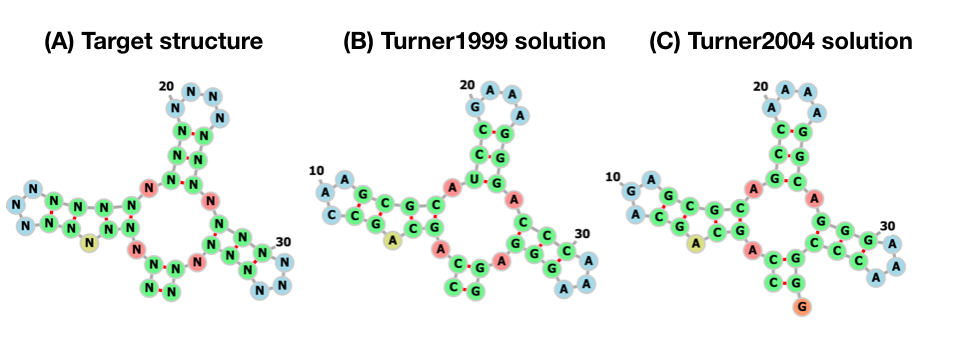
\includegraphics[width=1.0\linewidth]{../res/images/arnaque/fig9.png}
	\caption{\textbf{\texttt{aRNAque}'s performance on a TRIPOD secondary structure}. (A) The tripod target structure. (B) \texttt{aRNAque}'s solution using the Turner1999 energy parameter sets. (C) \texttt{aRNAque}'s solution using the Turner2004 energy parameter sets.}
	\label{Fig:tripod}
\end{figure*}
\subsubsection{\texttt{aRNAque} performance on a tripod secondary structure}

Finally, we performed a benchmark on a tripod target secondary structure. The tripod secondary structure was used as a third test case in the work of Ivry et al. \cite{ivry2009image}, and it does not contain any pseudoknot interactions. It comprises four stems, three of which with terminal hairpins, surrounding a multibranch loop (See Figure \ref{Fig:tripod}A). The tripod target structure was proved to be very challenging, especially because of its multiloop component, which is also found in some of the unsolved \texttt{Eterna100} target structures. We perform here, for both energy parameters \texttt{Turner1999} and  \texttt{Turner2004}, $100$ independent designs, using a population size of $100$ RNA sequences and a maximum of $5000$ generations. The mutation parameters used are: $P_{\mathcal{C}}=\{0.4,0.5,0.1,0,0,0\}$, $P_{\mathcal{N}}=\{0.7,0.1,0.1,0.1\}$ and $c=1.5$. When using the \texttt{Turner2004} energy parameter set, none of the $100$ designed RNA sequences was successful (i.e, $0$ sequence folds exactly into the target structure after $5000$ generations). Figure \ref{Fig:tripod}B shows one of the best solutions obtained out of $100$ designed sequences when using the \texttt{Turner2004}, the designed sequence folds into a structure at one error base-pair distance from the target structure. In contrast, when using the \texttt{Turner1999} energy parameters, we successfully designed the tripod secondary structure (See Figure \ref{Fig:tripod}C). The $100$ sequences designed folded exactly into the target structure with an average median number of generations $20$. When comparing both solutions to the one obtained in \cite{ivry2009image}, \texttt{aRNAque} (with no need of changing the RNA structure distance) can successfully design the multibranch loop component with one base pair error using the \texttt{Turner2004} energy parameter whereas \texttt{RNAinverse} (with the DoPloCompare distance) failed to design the multibranch loop, and the solution was at $2$ base-pair distance error.

\subsection{\texttt{aRNAque}'s performance on pseudoknotted target structures }
Secondly, we assessed the performance of \texttt{aRNAque} in designing pseudoknotted target secondary structures through intensive benchmark on \texttt{PseudoBase++} dataset. We then compared the results obtained to the one of \texttt{antaRNA}, using both folding tools \texttt{Hotknots} and \texttt{IPknot}. Furthermore, a comparison between local and Lévy mutations is provided.
\subsubsection{Best mutation parameter analysis on \texttt{PseudoBase++}: Levy mutation \emph{vs.} local mutation}
The advantage of using a Lévy mutation is its capacity to allow simultaneous search at all scales over the landscape. The search at different scale is often dictated by the exponent parameter of the heavy-tailed distribution. In this first subsection, we analyse for $80$ pseudoknotted target structures and for both mutation schemes the distributions of the best mutation parameters.
\begin{itemize}
	\item Binomial mutation: From Figure \ref{Fig:histomut}B, the critical range was identified to be from $0$ to $0.2$ and as $\mu$ becomes greater than $0.1$, the success rate decreases and the average number of generations increases. For each of the $80$ target structures with pseudoknots, $20$ sequences were designed for $\mu \in [0,0.2]$ with a step size of $1/L$. Figure \ref{Fig:tunning}B shows the histogram of the best mutation rate found for each target structure. Two main regimes are apparent: one where the best mutation rate is very low mutation rate ($\approx 1/L$) and another where the high mutation rate is optimal.
	
	\item Lévy mutation: From Figure \ref{Fig:histomut}C, the critical range of $c$ was identified to be $[1,2]$. For $c \in [1,2]$ and a step size of $0.1$, an optimum exponent parameter $c^*$ was investigated for all the $80$ target structures. Figure \ref{Fig:tunning}A shows the histogram of $c^*$. Contrary to binomial mutation, the optimum exponent parameter does not vary too much ($\forall \mathcal{S}$, $c^*\approx 1$).
\end{itemize}
Figure \ref{Fig:tunning} shows that when using a Lévy mutation, the optimal mutation rate is the same for most target structures. In contrast, the optimum binomial mutation rate parameter $\mu^*$ mostly varies with different targets. Although both mutation schemes (for the best mutation parameters) have approximately the same success rates, the Lévy flight mutation scheme is more robust to different targets. %Moreover, the median number of generations for the Lévy mutation is lower ($54$ for the Lévy and $92$ for the binomial mutation mode), thus enhancing efficiency.}

\begin{figure}[H]
	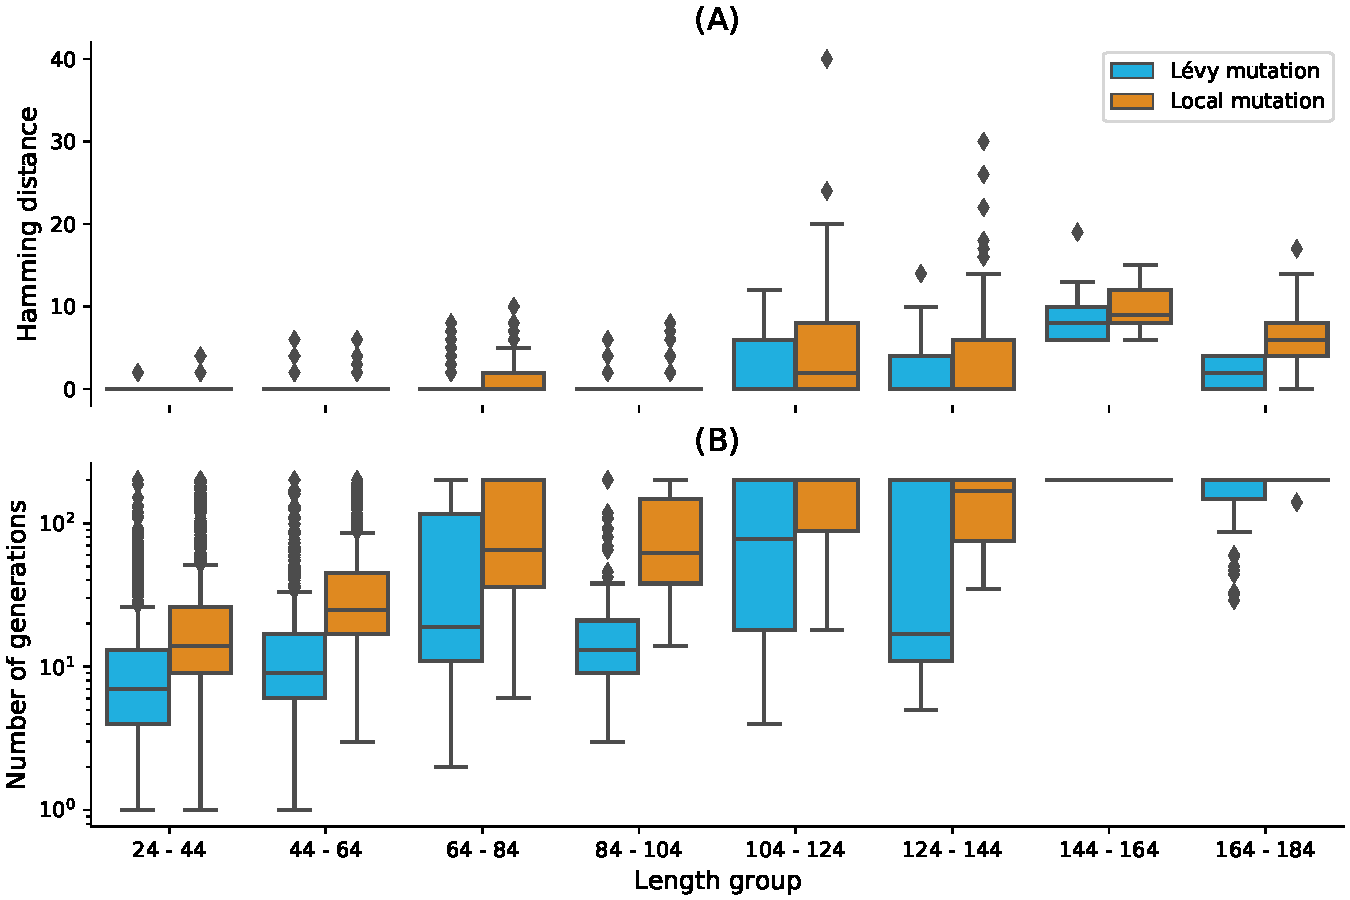
\includegraphics[width=1.0 \linewidth]{../res/images/arnaque/fig4.pdf}
	\small \caption{\textbf{Lévy mutation mode \emph{vs} local mutation (one-point mutation)}. (A) Hamming distance distributions \emph{vs.} target structure lengths. (B)  Number of generations distributions for different length groups. In both (A) and (B), lower values indicate better performance. The target structures are solvable in less than $100$ generations for both mutation schemes and most length groups. Still, the difference in the number of generations gets more significant as the target lengths increase, except for the two last length groups for which both mutation schemes mostly failed. The highest difference in terms of median number of generations is $150$ for target lengths in the range $[124-144]$ (respectively $123, 49, 46, 16, 7, 0, 0$ for the length ranges $[84-104], [64-84], [104-124], [44-64], [24-44], [144-164], [164-184]$). Averaging over all length groups, the median number of generations difference between the Levy mutation and the one point mutation is $48$ generations. }\label{Fig:OP_vs_aRNAque}
\end{figure}
\subsubsection{Performance on \texttt{PseudoBase++}: Levy mutation \emph{vs.} local mutation}
Figure \ref{Fig:OP_vs_aRNAque} shows box plots for the base pair distance (Hamming distance) and the number of generations for increasing target lengths under our two mutation schemes: binomial at low mutation rate (or one point mutation) and the Lévy mutation. For each pseudoknotted RNA target structure in the \texttt{PseudoBase++} dataset, we designed $20$ sequences.  The results show that using the Lévy mutation instead of a local mutation scheme can significantly increase the performance of \texttt{aRNAque}.  The gain was less significant in terms of designed sequences quality  (base pair distance distributions, with a $t$-value $\approx -1.04$ and $p$-value $\approx 0.16$) but more significant in terms of the average number of generations needed for successful matches to target structures (with a $t$-value $\approx -3.6$ and $p$-value $\approx 0.0004$). This result demonstrates a substantial gain in computational time when using a Lévy mutation scheme instead of a purely local mutation.

\begin{figure*}[t!]
	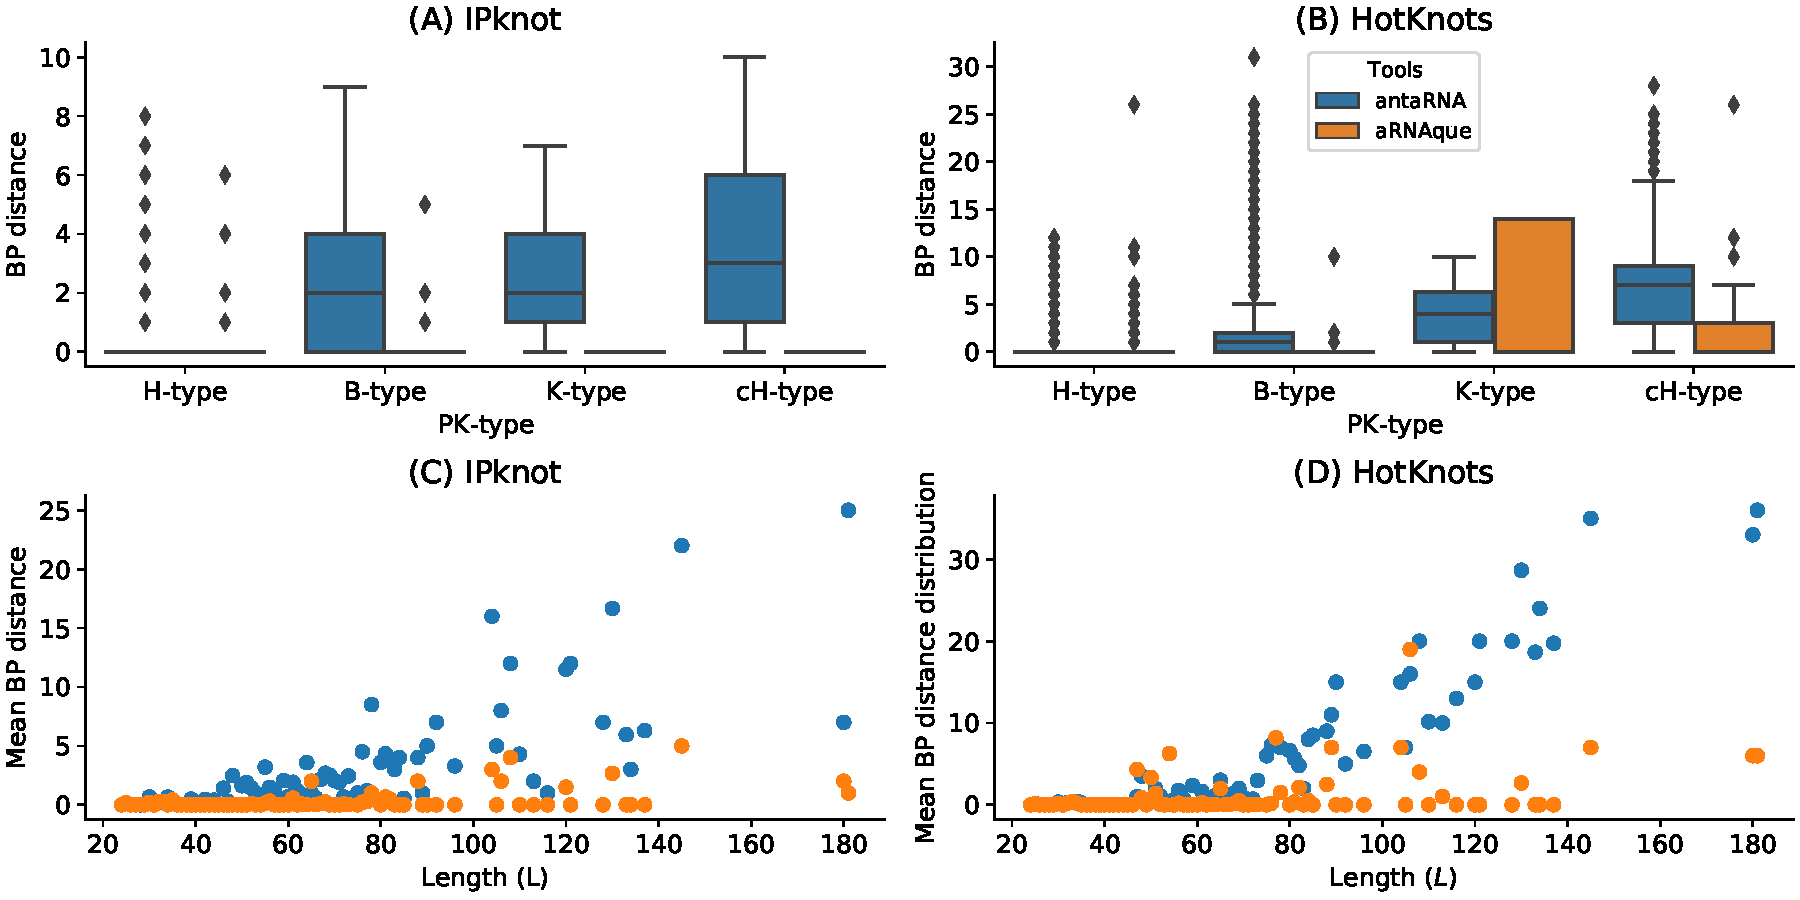
\includegraphics[width=1.0\linewidth]{../res/images/arnaque/fig5.pdf}
	\caption{\textbf{\texttt{aRNAque} \emph{vs} \texttt{antaRNA} on \texttt{PseudoBase++} dataset using both  \texttt{IPknot} and \texttt{HotKnots}}. Lower values imply better performance. (A, B) Base pair distance distributions of the designed sequences to the target structure for different pseudoknot types. (C,D) Mean base pair distance against target lengths. }\label{Fig:antaRNA_vs_aRNAque}
\end{figure*}
\subsubsection{Performance on \texttt{PseudoBase++}: \texttt{aRNAque} \emph{vs.} \texttt{antaRNA}}
%\subsubsection{General performance analysis using both \texttt{Hotknots} and \texttt{IPknot}}
We also compared the sequences designed using \texttt{aRNAque} (with the Lévy mutation scheme) to those produced by \texttt{antaRNA}. Figures \ref{Fig:antaRNA_vs_aRNAque}A and \ref{Fig:antaRNA_vs_aRNAque}C show the base pair distance distribution for each category of pseudoknotted target structure and the mean of the base pair distance plotted against the length of the target secondary structures. For \texttt{antaRNA}, and when using \texttt{IPknot} as a folding tool, finding sequences that fold into the target becomes increasingly difficult with pseudoknot complexity (median base-pair distance distribution increases). On the other hand, \texttt{aRNAque}’s performance improves as pseudoknot complexity increases (e.g. the mean base-distance decreases with the pseudoknot complexity). 
%In sum, as target length increases, the performance of \texttt{antaRNA} (local search) is considerably degraded , while \texttt{aRNAque} (Lévy flight search) stays almost constant.

A second benchmark using \texttt{HotKnots} as a folding tool was performed on the same dataset. For both \texttt{aRNAque} and \texttt{antaRNA}, the more complex the pseudoknot motifs, the worse is the tool performance (median of the base-pair distance distribution increases). Figures \ref{Fig:antaRNA_vs_aRNAque}B and \ref{Fig:antaRNA_vs_aRNAque}D show the base pair distance distributions with respect to the pseudoknot motifs for both \texttt{aRNAque} and \texttt{antaRNA}. Even though both performances degrade as target length increases, \texttt{aRNAque} (Lévy flight evolutionary search) performance remains almost constant for all the target lengths greater than $60$.
\subsection{Quality of the designed RNA sequences}
In addition to the successful rate analysis, we assessed the quality of the designed RNA sequences by analysing both GC-content and diversity of the pseudoknotted dataset using \texttt{IPknot}. This section presents the results obtained and a comparison to \texttt{antaRNA} designed sequences. 
\subsubsection{GC--content analysis of the designed sequences using \texttt{IPknot}}
The GC--content of an RNA sequence $S$ measures the concentration of G-C nucleotide in $S$ and influences its stability and biological function. Therefore, the ability of an inverse folding tool to control the GC--content is of vital importance for designing functional RNA sequences. Both \texttt{antaRNA} and \texttt{aRNAque} allow to control the GC--content at different levels of the optimization process: \texttt{aRNAque} through the mutation parameters $P_{\mathcal{C}}$ and $P_{\mathcal{N}}$; \texttt{antaRNA} with the parameter $tGC\in [ 0,1 ]$. In this section, we compare the performance of each tool for fixed GC--content values and analyse each tool's ability to control the GC--content. For each pseudoknotted target structure in the \texttt{PseudoBase++} dataset, four different GC-content values $\{0.25,0.5, 0.75, 1\}$, a poll of $20$ sequences is designed using \texttt{IPknot} as folding tool. That results in $5320$ designed sequences for each GC-content value and tool. The number of successes is the total number of sequences that fold exactly into the given target structure (i.e. the designed sequence folds into a structure at base-pair distance $0$ from the target structure). Figure \ref{Fig:GC_content} shows respectively the base pair distance distributions, the GC distance distributions and the number of successes for both \texttt{aRNAque} and \texttt{antaRNA}. The results show that the performance (in terms of success number) varies considerably with the GC--content values for both tools, and the best performance is obtained for both tools with a GC--content value of $0.5$. When comparing the GC-content distance (i.e absolute value of the difference between the targeted GC--content and the actual GC--content values of the designed sequences) distributions, both GC--content distance median distributions increase, whereas \texttt{antaRNA} controls significantly better the GC-content (See Figure \ref{Fig:GC_content}B). On average, for the respective GC-content values $\{0.25, 0.5, 0.75, 1\}$, \texttt{antaRNA}'s sequences have respectively $0.2569, 0.4952, 0.7314, 0.8684$ whereas  \texttt{aRNAque}'s sequences have respectively $0.3649, 0.4910,$ $ 0.6231, 0.811$; the main difference is at fixed GC-content values $0.25$ and $0.75$. Even though \texttt{antaRNA} designs sequences with better control of the GC-content, the gap in success rate still remains remarkable compared to \texttt{aRNAque}(See Figure \ref{Fig:GC_content}A and Figure \ref{Fig:GC_content}C).
\begin{figure*}[t!]
	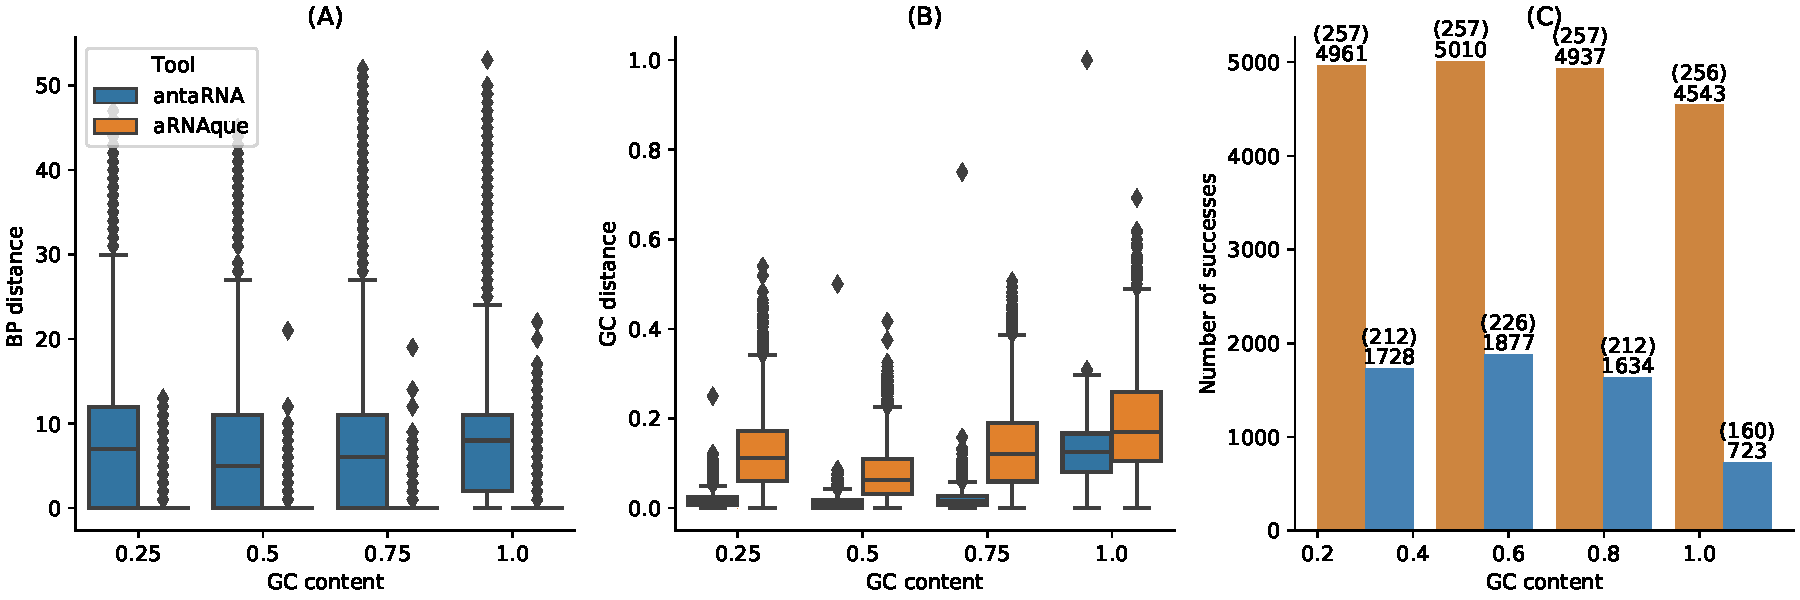
\includegraphics[width=1.0\linewidth]{../res/images/arnaque/GC_content.pdf}
	\caption{\textbf{\texttt{aRNAque} \emph{vs} \texttt{antaRNA} on \texttt{PseudoBase++} dataset using \texttt{IPknot}: GC--content analysis}. (A) Base-pair distance ditributions. (B) GC--content distance distributions. The difference betwen the targeted GC-content and the actual GC-content values. In (A,B), lower values imply better performance. (C) Number of successes realised by both inverse folding tools. Two values are considered: the up value represent the number targets successfully solved for each GC-content value out of the $266$ targets benchmarked; the down values represent the number sequences folding into the targeted secondary structure.}\label{Fig:GC_content}
\end{figure*}
\subsubsection{Diversity of the designed sequences}
Another advantage of using a Levy mutation when designing RNA sequences is to increase the chance of designing sequences with high diversity. Here, we use the positional entropy of each pool of $20$ sequences previously designed for each pseudoknotted target structure to compare the diversity of RNA of both tools \texttt{antaRNA} and \texttt{aRNAque} (Lévy search). We also compare it to the diversity of the designed sequences using the old version of \texttt{aRNAque} (Local search). The results show that the sequence diversity of both \texttt{antaRNA} and \texttt{aRNAque} (Lévy search) varies with the GC--content values, where the more diversified pool of sequence is achieved with a GC--content value of $0.5$. When comparing the pool of designed sequences with highest entropy (i.e. with a fixed GC-content of $0.5$) to the one of the old version of \texttt{aRNAque} (Local search), the \texttt{aRNAque} (Lévy search) and \texttt{antaRNA} produce sequences with similar entropy (i.e. with a median entropy of $61.01$ for Lévy search respectively $59.65$ for \texttt{antaRNA} (see Figure \ref{Fig:result_diversity}), whereas the entropy of the sequences designed using the Local search is lower. For the three others fixed GC-content values (i.e. $\{0.25, 0.75, 1 \}$, \texttt{aRNAque} (Lévy search) produces sequences with the highest entropy (respectively a median entropy of $58.9, 60.08, 51.52$ against  $53.42, 54.63, 48.38$ for \texttt{antaRNA}).
%In summary, the updated version of \texttt{aRNAque} (Lévy search) allows designing RNA sequences of high diversity with . 
\begin{figure*}[ht]
	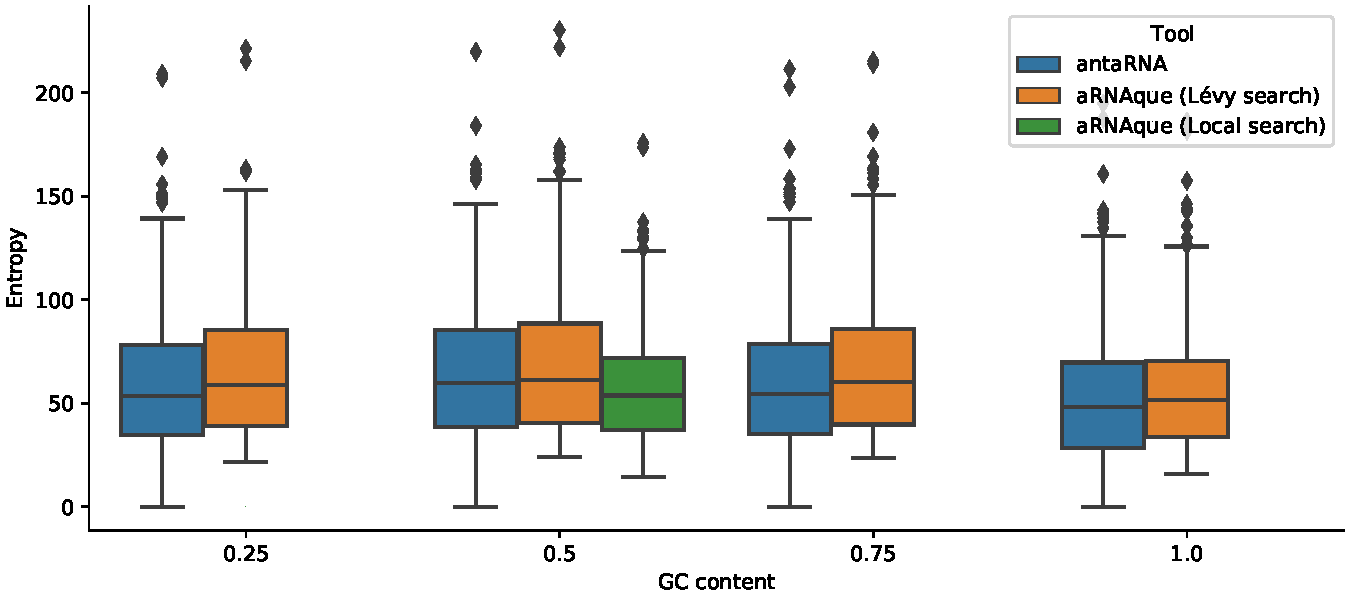
\includegraphics[width=1.0\linewidth]{../res/images/arnaque/fig7.pdf}
	\caption{\textbf{\texttt{aRNAque} \emph{vs} \texttt{antaRNA} on \texttt{PseudoBase++} dataset using \texttt{IPknot}: Diversity analysis}. The positional entropy distributions plotted agains the targeted GC--content values.  Higher values imply better performance.}\label{Fig:result_diversity}
\end{figure*}


\begin{figure}[t!]
	\begin{center}
		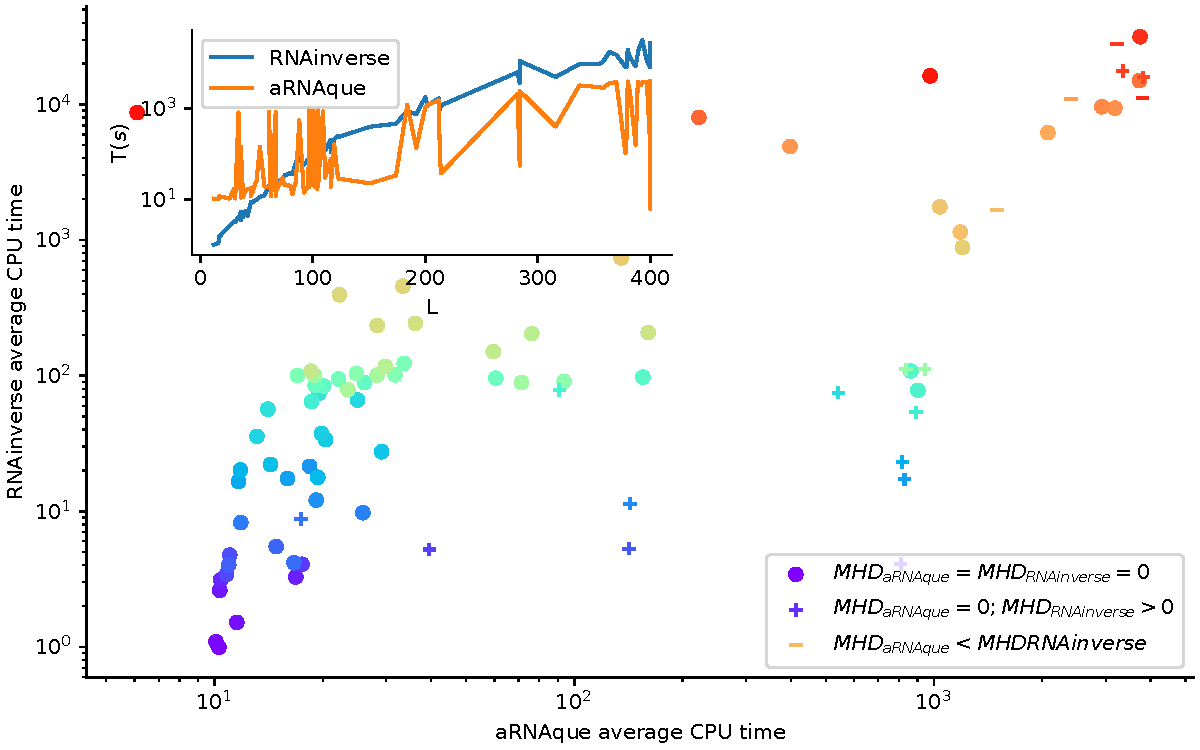
\includegraphics[width=0.98\columnwidth]{../res/images/arnaque/cpuvssuccess.pdf}
		\caption{\textbf{CPU time: \texttt{RNAinverse} $vs.$ \texttt{aRNAque}}. Each bubble corresponds to a target structure in \texttt{EteRNA100} dataset and, their colours are proportional to the length of the targets. In the legend, MHD stands for Median Hamming distance, and the different markers represent---('o') $100\%$ success for both tools---('+') $100\%$ success for \texttt{aRNAque} and not for \texttt{RNAinverse}---('-') for the case both tools fail to find at least one sequence that folds into the target. Underlying the CPU time difference is the inside plot that shows the CPU time (in seconds) as a target length function.}
		\label{719148}
	\end{center}
\end{figure}
\subsection{Complexity and CPU time comparison}
{\label{sec:complexity}}
We finally analysed the design performance of \texttt{aRNAque} relatively to the CPU time needed. This section presents \texttt{aRNAque} statistical results compared to two main tools: \texttt{RNAinverse} for the pseudoknot-free targets and \texttt{antaRNA} for the pseudknotted targets. 
\subsubsection{CPU time \emph{vs.} success rate using \texttt{RNAfold}:  \(\texttt{RNAinverse}\) vs. \(\texttt{aRNAque}\) on \texttt{EteRNA100-V1}. } 
Since our previous benchmarks on~\(\texttt{EteRNA100-V1}\) using the Turner2004 energy's parameters reveal that \texttt{RNAinverse}, one of the oldest inverse folding tools, stands behind \texttt{aRNAque} solving $66\%$ of the dataset; we have chosen to compare its computational time to our implementation (See Table \ref{Tab:eterna}).
The inset of the Figure {\ref{719148}} shows the CPU time in seconds needed to design for each target in the \(\texttt{EteRNA100-V1}\), \(5\) sequences. As the \(\texttt{RNAinverse}\) time increases exponentially with the length of the target, the \(\texttt{aRNAque}\) one does not. 

When comparing the ratio between the success rate and CPU time, \texttt{aRNAque}  mostly succeeded in finding at least one sequence that folds to the target with lower CPU time costs for average target lengths. In contrast, \texttt{RNAinverse} accuracy is lower, and the CPU time is expensive. The increase in CPU time may be because of the use of the partition function as the objective function.


\subsubsection{CPU time \emph{vs.} success rate using \texttt{Hotknots}: \(\texttt{antaRNA}\) vs. \(\texttt{aRNAque}\) on \texttt{PseudoBase++}}
We also compare \texttt{aRNAque}'s computational time to the one of \texttt{antaRNA}. For both tools, $20$ sequences were designed for each target structure of the \texttt{PseudoBase++} dataset. The GC--content value used for both tools is $0.5$, and the maximum number of interactions for  \texttt{antaRNA} is $5000$. 
Figure {\ref{fig:cputime_hotknots}} shows the median CPU time of the $20$ runs in seconds for both tools plotted against each other. We analysed the CPU time by partitioning the data into three groups: 1) a set for which both tools have a median base-pair distance of 0 ($158$ entries marked with o); 2) another set for which \texttt{aRNAque} has a median base-pair distance is 0 and \texttt{antaRNA} ($41$ entries marked with +); 3) the last set for which \texttt{antaRNA} designs are of better quality ($9$ entries mark as -). For the first group, we can notice that for most targets of short length \texttt{antaRNA} is faster than \texttt{aRNAque}. For the second group, although \texttt{antaRNA} average CPU time remains smaller, \texttt{aRNAque}'s success rate outperformed \texttt{antaRNA}.  On the one hand,  \texttt{aRNAque} average CPU time is higher than the one of \texttt{antaRNA}, but this could be due to its population-based algorithm, which often allows for designing more successful sequences. On the other hand, \texttt{antaRNA} is faster but less successful. Increasing \texttt{antaRNA}'s number of iterations will indeed increase the CPU time, but it may improve the quality of the designed sequences.

\begin{figure}[t!]
	\centering
	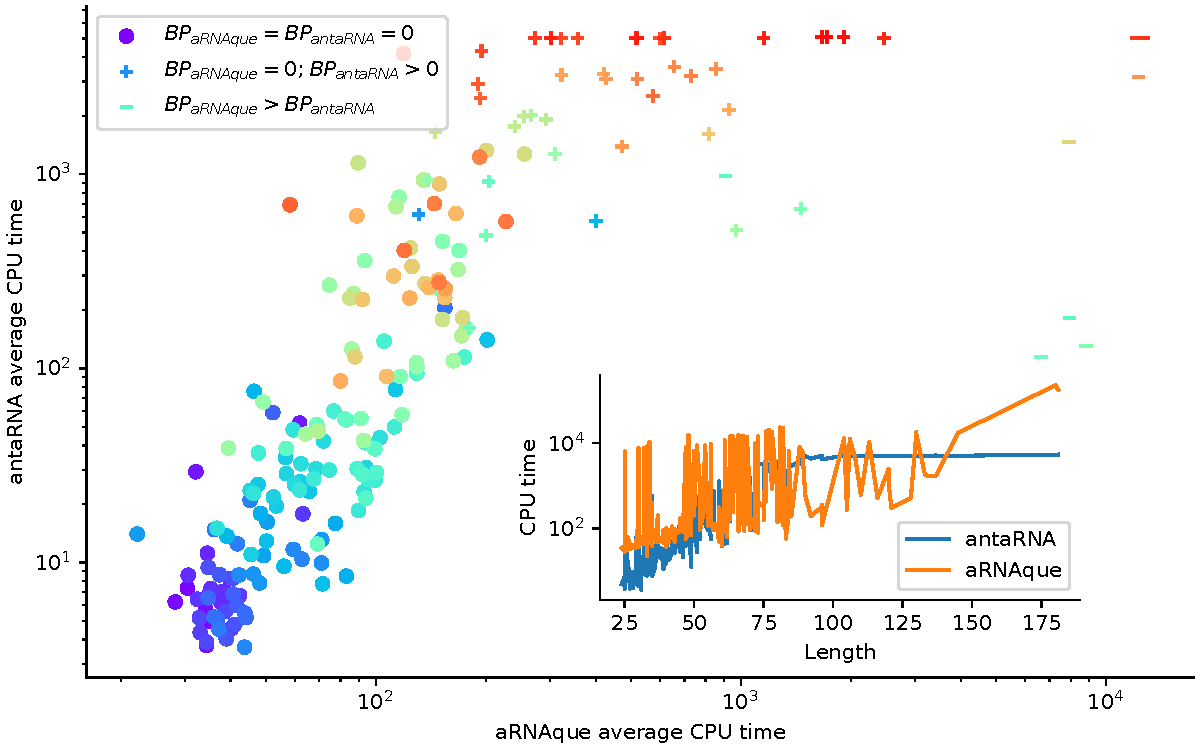
\includegraphics[width=1.0\linewidth]{../res/images/arnaque/CPU_time_Hotknots.pdf}
	\caption{\textbf{CPU time analysis using \texttt{Hotknots}: \texttt{antaRNA} $vs.$ \texttt{aRNAque}}. Each bubble corresponds to a target structure in \texttt{PseudoBase++} dataset and, their colours are proportional to the length of the targets. In the legend, BP stands for Median base pair distance, and the different markers represent---('o') $100\%$ success for both tools---('+') $100\%$ success for \texttt{aRNAque} and not for \texttt{antaRNA}---('-') for the case \texttt{aRNAque}'s desinged sequences are of median base pair distances greater than the one of \texttt{antaRNA}. Underlying the CPU time difference is the inside plot that shows the CPU time (in seconds) with respect to the target length.}
	\label{fig:cputime_hotknots}
\end{figure}

\section{Conclusion}
In this work, we investigated an evolutionary approach to improve the existing solutions to the RNA inverse folding problem. As a result, we proposed a new EA \texttt{python} tool called \texttt{aRNAque}.  \texttt{aRNAque} implements a Lévy flight mutation scheme and supports pseudoknottted RNA secondary structures. The benefit of a Lévy flight over a purely local (binomial with $\mu<<1$ or a single point mutation) mutation search allowed us to explore RNA sequence space at all scales. Such a heavy-tailed distribution in the number of point mutations permitted the design of more diversified sequences.

Our results show general and significant improvements in the design of RNA secondary structures compared to the standard evolutionary algorithm mutation scheme with a mutation parameter $\approx 1/L$, where $L$ is the sequence solution length. Lévy flight mutations lead to a greater diversity of RNA sequence solutions and reduce the evolutionary algorithm’s number of evaluations, thus improving computing time. 
